\documentclass[10pt, a4paper, conference, compsocconf]{IEEEtran}

% *** GRAPHICS RELATED PACKAGES ***
%
\ifCLASSINFOpdf
\usepackage[pdftex]{graphicx}
% declare the path(s) where your graphic files are
% \graphicspath{{./pics/}}
% and their extensions so you won't have to specify these with
% every instance of \includegraphics
% \DeclareGraphicsExtensions{.pdf,.jpeg,.png}
\else
% or other class option (dvipsone, dvipdf, if not using dvips). graphicx
% will default to the driver specified in the system graphics.cfg if no
% driver is specified.
% \usepackage[dvips]{graphicx}
% declare the path(s) where your graphic files are
% \graphicspath{{../eps/}}
% and their extensions so you won't have to specify these with
% every instance of \includegraphics
% \DeclareGraphicsExtensions{.eps}
\fi

% correct bad hyphenation here
\hyphenation{op-tical net-works semi-conduc-tor}


\begin{document}
%
% paper title
% can use linebreaks \\ within to get better formatting as desired
\title{CO600 - Technical Report}


% author names and affiliations
% use a multiple column layout for up to two different
% affiliations

\author{\IEEEauthorblockN{Bradley Jones}
  \IEEEauthorblockA{bj59@kent.ac.uk}
  \and
  \IEEEauthorblockN{Jack Fletcher}
  \IEEEauthorblockA{jpf4@kent.ac.uk}
  \and
  \IEEEauthorblockN{John Davidge}
  \IEEEauthorblockA{jd389@kent.ac.uk}
  \and
  \IEEEauthorblockN{Sam Betts}
  \IEEEauthorblockA{sab50@kent.ac.uk}
}

% make the title area
\maketitle

\newpage

\begin{abstract}
In this paper we will discuss the motivations for and the development of Project
Apiary - an end-to-end solution for real-time monitoring and analysis of log
data in distributed computer systems. In the development of Project Apiary we
explore the many problems associated with the gathering, storage and analysis of
schema-less data, and seek to define user-friendly approaches for processing,
and visualising this data. We also explore methods allowing the system to prompt
the user to act on important events as they happen, rather than discovering them
in an after-the-fact analysis.
\end{abstract}

%\begin{IEEEkeywords}
%  component; formatting; style; styling;
%
%\end{IEEEkeywords}

\IEEEpeerreviewmaketitle


\section{Introduction}

Data centres - which are collections of computers connected over a local area
network (LAN) - produce vast quantities of data in the form of application and
machine logs. The larger the data centre and the more complex its
applications, the larger the volume of data produced. With the ongoing
industry moving towards “cloud” computing, data centres are becoming ever
larger and being used for a wider variety of applications, often by thousands
or even tens of thousands of users simultaneously. The logs produced by the
services running on the machines which comprise the data centre contain a wide
range of generic (CPU loading, RAM usage, network traffic, etc) and
application-specific data which can be analysed to gain valuable insight into
the operation of the data centre. However, this data is usually unstructured
and unorganized - making meaningful analysis a non-trivial task. When combined
with the sheer volume of data being produced by ever larger data centers, the
gathering and analysis of this data becomes an ever more difficult task.

Solutions already exist to combat this problem (as detailed in the
background section below), but many of these are closed-source and
expensive, and in our opinion those that are open-source do not currently
tackle every aspect of the problem in a complete end-to-end solution. Given
our background in open-source software we were motivated to explore the
development of an open-source project which covered every component
necessary for a user to gain meaningful insight into the workings of their
data centre.


\section{Project Background}

The four of us have been working together as a team since the beginning of our
Year In Industry at Cisco Systems in San Jose, California. During our time there
we gained valuable experience of working with both large and small distributed
computer systems - mainly focused in the world of open-source cloud computing.
In the course of our work we were exposed to various tools for the monitoring of
these distributed systems, but in all cases found them wanting in some respect.
Of the tools with which we came into contact we believe these to be the most
important:

\subsection{Splunk}

Splunk\cite{splunk} is probably the closest to an industry standard when it comes to
analysis of distributed systems. It is a large, enterprise-grade product capable
of solving most of the problems we set out to solve with Apiary. The problem
with Splunk is that it is expensive to use and is largely closed-source. This
does not fit with our philosophy on software transparency and is prohibitive for
those who cannot afford to pay.

\subsection{Elasticsearch ELK}

The Elasticsearch ELK\cite{elk} stack (Elasticsearch, Logstash, and Kibana) is
conceptually very similar to Apiary. It’s open-source and it consists of many
components working together to solve separate parts of the overall problem. A
major difference between Apiary and ELK is in the way that the components
communicate with each other. ELK uses a REST API to communicate over HTTP,
whereas Apiary makes use of a distributed message bus. We believe that this
solution is better for scalability and security.


\section{Aims}

The aim of Apiary was to produce an open source platform for the harvesting,
storage, processing, and visualisation of machine data (logs etc) from large
scale distributed systems, and expose this using a real time, interactive web
front end. In order to ensure that our project was successful, we set out a
series of clear defined goals before starting the project.

\begin{itemize}

\item Scalability - During our research we found that typical log rates for data
centre applications could run into terabytes per hour. This meant that we
would need to be able to handle more data than a single appliance could ever
store, and still maintain an acceptable level of service. For this reason
building a system that was easily scaled out was of paramount importance.

\item Real Time - We decided quite early on that we would be able to provide a
richer, more interactive service by building a system that operated on a
message based, real time system. This would allow us to push events from the
data center all the way to the browser without implementing costly polling
techniques.

\item Simple Configuration - A problem that we identified with a lot of open
source software stacks is that they are often very difficult to configure, and
come with hundreds of configuration options. This can make devops (developer
operations) very difficult, and just finding the optimal set of configurations
can be a task unto itself. For this reason we wanted to keep configuration
options to a minimum, and automatically detect configuration for as much of
the stack as we possibly could.

\item Alert System - One component that we noticed most of the existing
solutions don't have, is any kind of event alert system. The user cannot be
expected to be monitoring the system at all times, so we decided that we
should be able to push triggered alerts directly to the users mobile device.

\item User Friendly UI - Another thing we noticed about a lot of the existing
solutions out there, particularly those that were open source, was that UI was
often treated as a second class citizen to functionality. We wanted to ensure
that our UI was simple, easy to understand, and provided rich data
visualisations that allowed the user to gain the most from their data.

\item Powerful Query System - Our project has a wide range of applications, and
in order to support them all we needed to ensure that the query language could
support a wide range of simple and complex operations, whilst remaining fast
and real time.

Use cases for a system like this include live alerting of machine failures, or
heavy network load; analyzing browsing and buying patterns in e-commerce
websites from web server log data; and identifying network abuse by indexing
data from firewalls and intrusion detection systems.

\end{itemize}


\section{Architecture and Design}

In this section we will discuss the specific solutions that we built in order to
achieve our goals, the motivations behind our design decisions, and the
technical challenges we overcame. Our project ended up being divided into a
series of independent components; Bee, our data agent; Hive, responsible for
storage and processing of data; Queen, our web front end; and finally, our iOS
application.

\graphicspath{{./pics/}}
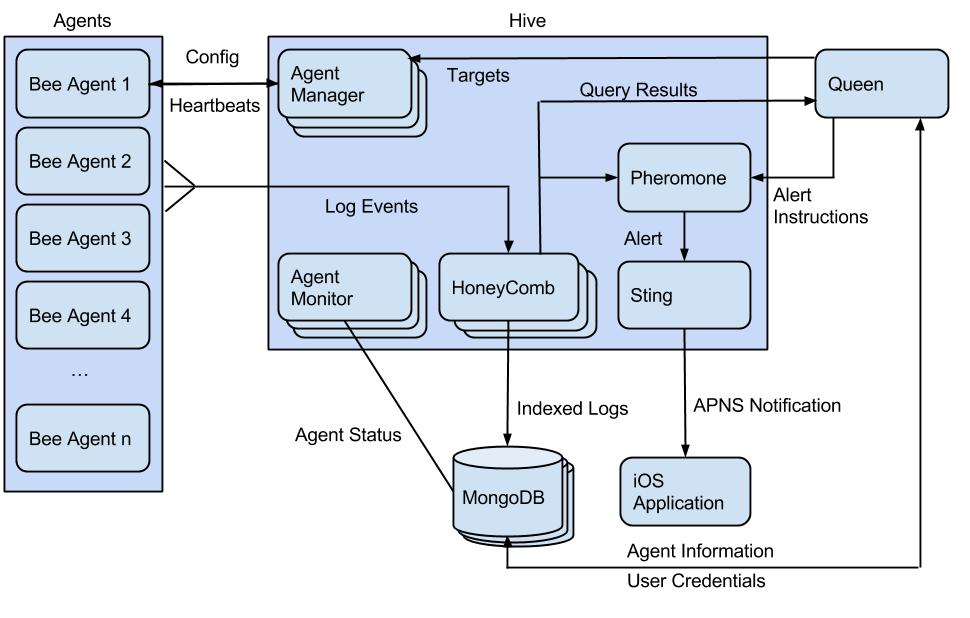
\includegraphics[width=\textwidth, keepaspectratio]{design.jpg}

The key design decision was to build our system in a ‘Process Oriented’ manner.
This meant all components were broken down into small, scalable components. All
state was stored in a central, scalable database, and all communication was
handled by a scalable RabbitMQ\cite{rabbit} messaging exchange. Designing the system in
this way meant that we could leverage these technologies to provide a reliable,
transparently scalable, and real time system.

The reasons for choosing RabbitMQ over other communication paradigms and
technologies, such as REST, were that it would provide automatic distribution of
messages across subscribers, giving us free load balancing and thus scaling. It
would also queue messages in the case of congestion, ensuring reliability, and
behaves in an event driven manner - allowing us to react in real-time to events
across the whole stack.

For the database we opted for MongoDB\cite{mongo}. We decided this was the best option
for the project because of the necessity to have very flexible data structures.
MongoDB stores collections of JSON objects instead of having rigid tables,
allowing for metadata and optional extra fields to be added dynamically to
objects - a feature that we specifically wanted for log entries. Due to the
lack of relations in MongoDB it is also known to scale very well, and because
MongoDB is JSON based like the rest of our stack, we would avoid data
consistency issues as no conversion would need to be performed between
components.


\section{Bee}

Bee is our data-harvesting agent, which is installed on all monitored machines
and forwards log data into Hive. We designed Bee to be as lightweight and easy
to set up as possible. This is because we wanted to ensure that Bees did not
interfere with the normal operation of the machine it was monitoring, and for
the initial installation task to be as trivial as possible.

For this reason Bee has only 1 configuration option - the IP of your central
RabbitMQ cluster. After that all other configuration is either automatically
discovered from the host machine (MAC address, hostname, etc), or received from
Hive after an initial handshake over the RabbitMQ exchange. After this, Hive can
request that this particular instance of Bee listens to and forwards changes to
any file on that particular machine.

Bee is based on NodeJS\cite{node}, as we needed it to be multi-platform, and the
event-driven nature of its framework lends itself well to file monitoring, as
well as responding to incoming RabbitMQ messages. It is designed using a
Model-View-Controller (MVC) framework, with a series of actions for different
commands from Hive.


\section{Hive}

Our core, and most complex component - its role is to manage data agents
(Bees), store incoming log data, and provide complex querying against that
data. In order to achieve scalability, Hive is made up of 6 subcomponents, with
a simple framework in place for extending this with extra components should the
user require additional functionality. All components communicate over the
RabbitMQ message exchange.

Given our background with OpenStack (written in Python) and the abundance of
bindings and support for many of the other technologies we wanted to employ,
Python was the obvious language choice for Hive. Python also provided a clean
multiprocessing library which was crucial for a number of subcomponents. We
chose to implement a common MVC stack for all our components, along with a JSON
protocol that would be shared across the whole stack. This allowed us to
rapidly prototype and add new components to Hive as all the communication
management and database access code were broken out into a reusable library.


\section{Hive Subcomponents}

\subsection{Agentmanager and Agentmonitor}

These were the first of the Hive subcomponents to be built, the purpose of
Agentmanager and Agentmonitor are to configure and keep track of our Data Agents
(Bee).

Agents are, as described earlier in the paper, installed with no configuration.
Agentmanager’s first job is to handshake new Agents entering the environment and
provide them a unique identifier which is attached to data transmissions to the
rest of Hive. After the initial bootstrapping of an Agent, Agentmanager then
receives periodic heartbeats from the Agents. This heartbeat is used by
AgentMonitor to detect the status of an Agent in the case of an unclean
disconnection, error, network congestion, or other problem with the host
machine.

The final task performed by these two components is to provide the Agents with a
series of Data targets, in the case of the file watching Agent, this allows a
user to remotely set the files that the Agent is monitoring. The API allows this
to be done in bulk, with many targets, across many Agents, to prevent
repetitiveness. Agent status responses (success, fail) are then collated and
returned in a labeled list.

Maintaining the real time aspect of the whole application required the addition
of “events” to Agentmanager and Agentmonitor. Whenever a significant change
happens on either component; such as, a new agent handshakes into the
environment, or an agent is flagged as dead, the component where this change
happened publishes an event object onto a known message exchange, which other
services - if they are listening - can use to perform any tasks they have which
are relevant to a change in the Agent Manager without the need for polling.
Subscription to this exchange is completely open, optional and will not alter
the overall behavior of the program.

The reason for splitting this component into both Agentmanager and Agentmonitor,
is because the tasks performed by each scale differently. Agentmanager needs to
handle a constant stream of Agent heartbeats, which get more frequent, as more
Agents are added. In comparison Agent Monitors’ task does not increase in
complexity as fast, and because of this, it does not need to be scaled as
aggressively. This configuration of split services provides the greatest
flexibility for host utilisation at large scale, as you can scale very specific
parts of the whole application.

\subsection{Honeycomb}

Honeycomb is our most complicated component as this is where all the storage and
processing of collected data takes place. Honeycomb follows the standard hive
component structure, and uses a common MVC stack for inbound requests. It uses a
subscriber queue to digest the stream of data it receives as fast as possible
without having to respond to each request, which would slow the process down.

Honeycomb uses our common model structure (see Common) to verify the validity of
all received data before it is saved to the database. There is also an
additional step in the Honeycomb save function to perform indexing for every
data entry. After some research we settled on using PyLucene\cite{pylucene} as a python
wrapper for Lucene\cite{lucene} to handle indexing. Lucene is an open-source plain text
analysis and search tool developed by the Apache Software Foundation. Whenever
data is saved it is passed to Lucene for indexing so that we can utilize their
powerful query syntax, without having to apply schema to the contents of the
data.

As well as storing the data, Honeycomb also exposes an API for searching it.
These searches can be one of two types; a one-off query, or a recurring query.
One-off queries are simply a remote procedure call (RPC) containing the query.
The response is written into a JSON object and passed back to the requesting
process via the message bus. This is great for individual tasks, but in order to
facilitate real time updates we needed to introduce recurring queries. Recurring
queries require a little more setup as they need to be run concurrently
alongside the main Honeycomb thread. Since Honeycomb has to remain stateless for
scalability, it should not locally maintain any reference to these background
threads, as this would mean that a second instance of Honeycomb wouldn’t be able
to interact with the new query.

In order to solve this issue we use the message bus again, spawning a wrapper
process which provides an API to the thread in the background, and stores the
key to communicate with that wrapper process in the database. The recurring
query thread isn’t complex, simply running the lucene query then waiting a
second before running it again. The thread also maintains a list of any
previously discovered log IDs, and will only output if there has been a change,
or if it has been asked to send the next set of results. Output for these
background queries is pushed onto a uniquely named fanout exchange on the
message bus. This allows multiple processeses to receive copies of the output
from a single query, and also ensures that if no one is listening the output is
simply thrown away instead of clogging up a queue on the message bus.

\subsection{Pheromone}

Using the recurring query API in Honeycomb, Pheromone places a layer of
intelligence on top of the query to filter out specific results and trigger
alerts based on user-defined conditions. Alerters are created through the
Pheromone API. These alerters take trigger cases, and search parameters they
need to test for an alert, and a custom message that is included when an alert
is transmitted. Pheromone currently only has the one type of alerter - it will
fire an alert if a query gets a certain number of matches during a given
timescale. However it is not limited to just this one alert type, as the design
patterns used for the alerters allows for easy addition of new ones in the
future.

Pheromone uses python's multiprocessing library to start background tasks
similar to how Honeycomb’s recurring query tasks operate. When a request comes
in Pheromone starts a new alerter in the background, however unlike the
Honeycomb workers there is no unique output exchange, as alerts are always
pushed onto a known message bus routing key. This allows other services, for
example Sting, to listen for them and perform all necessary tasks they have
relative to the alert.

\subsection{Sting}

Pheromone alerts are a very powerful tool, but the user is not always going to
be sitting in front of their computer when an alert is triggered. In fact, the
very nature of user-defined alerts generally makes the times when they will
occur rare and/or unpredictable, and so we must be able to inform the user of an
alert as reliably as possible. By building a native iOS\cite{ios} app as described
later in this paper, we are able to take advantage of the Apple Push
Notification Service (APNS)\cite{apns}. APNS is a service made available by Apple to
all iOS application developers for sending small text-based messages to iOS
devices using your mobile application. In many ways this is similar to the
standard Short Message Service (SMS), but with the key differences that the
message is sent specifically to the application on the device, and more
importantly - is free. Many third-party services exist for sending automatically
triggered SMS messages (for example, Twilio\cite{twilio}), but these services charge
several pence per message, which could become very expensive in a large system
with many users and alert conditions.

When Pheromone pushes an alert onto the message bus, Sting picks it up and
looks up the user to which the alert is registered. For every iOS device
registered to that user (multiple iPhones, iPads, etc.) Sting will generate an
APNS push notification using the alert text specified by the user and the
Device ID associated with the device. The messages are then sent using the
APNS API - typically taking up to 5 seconds to arrive. This system ensures
that a user will always receive potentially critical updates about the state
of their system as and when they happen, giving them the time to act on them
before it may be too late.

\subsection{Common}

Though not technically a subcomponent in itself - Common is the base layer
underlying almost all of the hive subcomponents. Any code that was duplicated
and was reusable was moved into Common to maintain the DRY\footnote{Don’t Repeat Yourself} programming style.
Common therefore became the home for our MVC stack, including the parent classes
associated with writing controllers and routers. Common also includes drivers
for generic database access, meaning that the underlying database technology
could be changed fairly trivially if necessary. The current model uses
PyMongo\cite{pymongo} to hook into MongoDB.

The Base program pulls all the these parts together into an application that
runs but needs extending to provide any real functionality. It handles the
loading of configuration files and makes sure they are accessible throughout the
rest of the program. It also spawns the worker threads required to listen on the
message bus. Both a subscriber queue and worker queue are listened to in order
to distinguish between RPC (remote procedure call) messages which always require
a response, and purely informative messages - which require action but no
response. Base also sets up and handles all the logging throughout the program,
ensuring that it gets written to an intuitively named file and in a common
format that makes issues easier to find.


\section{Queen}

Our front-end component, also built on the NodeJS framework pulls all of the
components of Hive together to provide a real-time, visually rich experience.

We used the express library in NodeJS to build an MVC framework for the UI to
keep inline with our design style throughout the rest of the project. This has
lead to a clean, modular codebase that has very little duplication of code.
The most important decision designing Queen was to ensure that all data
transferred to the front-end would happen in real-time. In order to enable this
we took advantage of the socket.io library to have web-sockets that allow
client(front-end) to server(Queen back end server) communication.

Like the rest of our components Queen uses rabbit to provide inter-component
communication. The flow for communication with other components is described here
using a user performing a search as an example:

\begin{enumerate}
  \item The search terms are passed from the UI as a JSON object back to Queens
  server via a web-socket.
  \item Queen server then passes this data onto the appropriate Hive component
  via RabbitMQ, using either a remote procedure call or publish/subscribe model
  as appropriate.
  \item The Hive component (in this case Honeycomb) will then return the data to
  Queen server.
  \item The exact data that is required for the front-end is extracted and
  passed back up to the UI via a web-socket.
\end{enumerate}

If we request data using a publish/subscribe model, then every time the Queen
server receives data on the subscribe queue it can push that data back up to the
front-end using a web-socket. This means that the UI always has all of the
information available to it and the browser will not freeze as it would if we
were using a RESTful/polling approach to getting new data to the UI.

Queen enables multiple users to all be using the service at once. The principle
for multiple users is to store queries/alerts that the user wants to access next
time they use the system, also to store a list of Devices associated to the user
to be used by our iOS application. To store this data persistently Queen also uses
MongoDB.

Just as we did with the Bee/Agents we wanted to keep Queen configuration as
simple as we could. The configuration options as such are kept to just the IP
address of the rabbit server that all of the other components are talking on and
the IP address of the mongo server. By having the IP address of the mongo server
as a configuration option Queen can either be running its own mongo server or
use the existing one setup for Hive.

Rich visualisations were another main goal in designing Queen, due to our
experience using the d3js visualisation library we naturally decided to use
this. It has enabled us to use visualisations such as sparkline graphs to map
event rates in the system and pie charts to compare search results. From a
human computer interaction (HCI) point of view this gives the user access to the
same data in a more meaningful form, and that data can be accessed at a glance
rather than reading copious amounts of text to come to the same conclusion.

Due to the quantity of data that can come back from search results it was
important not only to visualise this in graph form but also allow users to
filter the actual log entries live in the browser opposed to sending of another
more refined query to Hive. In order to do this we put all data that we desire
to be searchable in a datagrid from the fuelux library which provides instant
searching for all data in the datagrid.

fielding stuff


\section{iOS Application}

In the real world a user will not always be sitting in front of their computer
when they need to know something about the computer system being monitored by
Apiary. However, it is likely that they will be carrying a modern smartphone
with them almost all the time, which will have a reasonably consistent WiFi or
cellular data connection. Due to our GUI being entirely web-based a user could
access everything they need to know using their smartphones web browser, but by
creating a native application we can enhance the user experience and provide
added functionality. A small but significantly useful function is the ability
to save the Apiary URL for the environment being monitored between invocations
of the application - speeding up a users access to the system. We can also save
the users login credentials for the same reason.

The greatest argument for a native application is the ability to exploit the
powerful Apple Push Notification System. As described above in the Sting
section, APNS can be used to send the user real-time updates on the status of
their computer system at anytime, as long as they have a cellular/WiFi data
connection. When a user logs into Apiary using the iOS application, their
unique Apple Device ID is registered against their user account to be used by
Sting for alert notifications.


\section{Future Work}

\subsection{Future Agents}

Very early on in our design we decided that our Agents system should be flexible
enough to accommodate a variety of agent types, as not all schemaless data comes
from text log files. We had the following Agents planned, but due to time
constraints were not able to implement them, and felt that our time would be
better spent focusing on processing techniques and UI.

First of all, given our OpenStack background, we would have liked to have built
an Agent that was integrated with OpenStack Ceilometer\cite{ceilometer}, the monitoring and
metrics component of OpenStack. This would have worked in much the same way, but
rather than have the user define a file, they would need to define a Ceilometer
Meter to start watching. After this event processing would have worked in
exactly the same way.

Another consideration was to build an Agent, or extend Bee so that it could tap
into popular logging frameworks. Many applications have now started to move away
from traditional log files, and instead pump data into logging frameworks which
can maintain slightly more structure about a log. Examples include
LogBack\cite{logback}, or Log4j\cite{log4j}.

Furthermore, other open-source projects could be extended to work with our
system, such as FluentD\cite{fluentd}, which has a plugin system that would allow us to
easily build in Apiary support.


\subsection{Hive - Timemachine and Intelligence}

Two future Hive components we considered but were not within the time scale of
the project were Timemachine and Intelligence.

Timemachine would be designed to pull data from the database according to a
query, and then push results onto a message queue in the same order and format
that they originally sent from the agents. A typical use case for this would be
an application that requires a replicated stream of historical data for playing
back events as they happened. This historical playback could be used to analyse
system faults to determine what went wrong.

Intelligence is much more complex and has potentially many more use cases. The
idea behind Intelligence is to provide an API for doing more advanced, deferred
data processing, such as Map Reduce tasks with the log data stored in
Honeycomb. Software like Hadoop\cite{hadoop} would allow for more in depth analysis than
is currently possible with the Lucene implementation in Honeycomb, but would
not work in real-time. The scope of Intelligence could potentially be extended
to include machine learning which we hope would compliment Pheromone with
dynamically generated alerts.


\section{Conclusion}

To conclude we set out to design and build an end-to-end solution for real-time
monitoring and analysis of log data, this we feel we have achieved
successfully. We had several goals which sculpted our design and thought
processes for the project, and we believe we have met them with the solution we
have built.

Scalability - Splitting the Hive into several components communicating via
RabbitMQ has given us industry-proven levels of scalability at zero cost and
with very little implementation overhead. The use of MongoDB has also given us
a database backend which has been tested to destruction in all corners of the
tech industry.

Real Time - RabbitMQ and web sockets have been used to create truly real time
communication between the many components of Apiary and the web front end.
Expensive polling loops are not required to keep the user up to date with the
state of their system.

Simple Configuration - Designing components such as the Bee to self-configure
based on data passed from the central Hive has made deploying Apiary across a
distributed system a much more straightforward task than many open source
projects. The inclusion of installation scripts has also contributed to this
goal significantly.

Alert System - Exploiting the real time nature of our message bus
infrastructure and the recurring query API exposed by Honeycomb has allowed us
to create the Pheromone and Sting componets. These components work together
with the iOS application to provide the user with real time feedback regardless
of their location.

User Friendly UI - Brad/Jack write something about graphing etc?

Powerful Query System - By exploiting the advanced text search language that
Lucene provides and combining this with fielding in Queen we have built a
system that allows the user to filter, and infer schema onto otherwise
unorganised data. Lucene's query language is expansive, and we ourselves are
yet to fully explore all of the features it provides.



% conference papers do not normally have an appendix


% use section* for acknowledgement
\section*{Acknowledgment}
The authors would like to thank the following people for their assistance during
the project:

Ian Utting - http://www.cs.kent.ac.uk/people/staff/iau

Debojyoti dutta - Cisco Systems, San Jose, CA

Lew Tucker - Cisco Systems, San Jose, CA

% trigger a \newpage just before the given reference
% number - used to balance the columns on the last page
% adjust value as needed - may need to be readjusted if
% the document is modified later
%\IEEEtriggeratref{8}
% The "triggered" command can be changed if desired:
%\IEEEtriggercmd{\enlargethispage{-5in}}

% references section

% can use a bibliography generated by BibTeX as a .bbl file
% BibTeX documentation can be easily obtained at:
% http://www.ctan.org/tex-archive/biblio/bibtex/contrib/doc/
% The IEEEtran BibTeX style support page is at:
% http://www.michaelshell.org/tex/ieeetran/bibtex/
%\bibliographystyle{IEEEtran}
% argument is your BibTeX string definitions and bibliography database(s)
%\bibliography{IEEEabrv,../bib/paper}
%
% <OR> manually copy in the resultant .bbl file
% set second argument of \begin to the number of references
% (used to reserve space for the reference number labels box)
\begin{thebibliography}{1}

  \bibitem{splunk}
    Splunk - http://www.splunk.com

  \bibitem{elk}
    Elasticsearch ELK - http://www.elasticsearch.org

  \bibitem{rabbit}
    RabbitMQ - https://www.rabbitmq.com

  \bibitem{mongo}
    MongoDB - https://www.mongodb.org

  \bibitem{node}
    NodeJS - http://nodejs.org

  \bibitem{os}
    OpenStack - https://www.openstack.org

  \bibitem{pymongo}
    PyMongo - http://api.mongodb.org/python/2.7rc0/

  \bibitem{pylucene}
    PyLucene - http://lucene.apache.org/pylucene/

  \bibitem{lucene}
    Lucene - http://lucene.apache.org

  \bibitem{ios}
    iOS - https://developer.apple.com/devcenter/ios/index.action

  \bibitem{apns}
    Apple Push Notification Service -
    https://developer.apple.com/library/ios/documentation/
    NetworkingInternet/Conceptual/RemoteNotificationsPG/
    Chapters/ApplePushService.html

  \bibitem{twilio}
    Twilio - https://www.twilio.com

  \bibitem{express}
    Express - http://expressjs.com

  \bibitem{socket}
    Socket.io - http://socket.io

  \bibitem{d3}
    d3js - http://d3js.org

  \bibitem{fuelux}
    FuelUX - http://exacttarget.github.io/fuelux

  \bibitem{ceilometer}
    Ceilometer - https://wiki.openstack.org/wiki/Ceilometer

  \bibitem{logback}
    Logback - http://logback.qos.ch

  \bibitem{log4j}
    Log4j - http://logging.apache.org/log4j/2.x/

  \bibitem{fluentd}
    FluentD - http://fluentd.org

  \bibitem{hadoop}
    Hadoop - http://hadoop.apache.org

\end{thebibliography}

% that's all folks
\end{document}
